
 \documentclass[12pt]{article}
\usepackage{graphicx}
\usepackage{booktabs}
 \usepackage{makecell}
 \usepackage{float}
 \newcommand{\diff}{\,\mathrm{d}}
\usepackage[margin=1in]{geometry}
\usepackage{fancyhdr}
\pagestyle{fancy}
\usepackage{extarrows}
\usepackage{breqn}

\newcommand{\N}{\mathbb{N}}
\newcommand{\Z}{\mathbb{Z}}
\newcommand{\trans}{^{\mathrm T}}
\usepackage{amssymb}
\usepackage[table]{xcolor}
\usepackage{bm}
\usepackage{array}
\usepackage{mathtools}
\usepackage[english]{babel}
\usepackage{natbib}
\usepackage{url}
\usepackage[utf8x]{inputenc}
\usepackage{amsmath}
\usepackage{graphicx}
\graphicspath{{images/}}
\usepackage{parskip}
\usepackage{fancyhdr}
\usepackage{vmargin}
\usepackage[font={bf, footnotesize}, textfont=md]{caption}
\usepackage{amsmath,amsthm,amssymb}


\newenvironment{theorem}[2][Theorem]{\begin{trivlist}
\item[\hskip \labelsep {\bfseries #1}\hskip \labelsep {\bfseries #2.}]}{\end{trivlist}}
\newenvironment{lemma}[2][Lemma]{\begin{trivlist}
\item[\hskip \labelsep {\bfseries #1}\hskip \labelsep {\bfseries #2.}]}{\end{trivlist}}
\newenvironment{exercise}[2][Exercise]{\begin{trivlist}
\item[\hskip \labelsep {\bfseries #1}\hskip \labelsep {\bfseries #2.}]}{\end{trivlist}}
\newenvironment{reflection}[2][Reflection]{\begin{trivlist}
\item[\hskip \labelsep {\bfseries #1}\hskip \labelsep {\bfseries #2.}]}{\end{trivlist}}
\newenvironment{proposition}[2][Proposition]{\begin{trivlist}
\item[\hskip \labelsep {\bfseries #1}\hskip \labelsep {\bfseries #2.}]}{\end{trivlist}}
\newenvironment{corollary}[2][Corollary]{\begin{trivlist}
\item[\hskip \labelsep {\bfseries #1}\hskip \labelsep {\bfseries #2.}]}{\end{trivlist}}
\DeclareMathOperator{\tr}{tr}
\DeclareMathOperator{\rank}{rank}
\DeclareMathOperator{\Span}{span}
\DeclareMathOperator{\row}{row}
\DeclareMathOperator{\col}{col}
\DeclareMathOperator{\range}{range}
\DeclarePairedDelimiterX{\inp}[2]{\langle}{\rangle}{#1, #2}
\DeclareMathOperator{\Proj}{Proj}
\DeclareMathOperator{\trace}{trace}
\newcommand{\Her}{^{\mathrm H}}
\DeclareMathOperator{\diag}{diag}
\makeatletter 
    \newcommand\fcaption{\def\@captype{table}\caption}
\makeatother
\setmarginsrb{3 cm}{2.5 cm}{3 cm}{2.5 cm}{1 cm}{1.5 cm}{1 cm}{1.5 cm}
\setlength\parindent{1em}

\title{Short Report: Large Amplitude Pendulum}                             % Title
\author{Chen Ang}                               % Author
\date{\today}                                           % Date

\makeatletter
\let\thetitle\@title
\let\theauthor\@author
\let\thedate\@date
\makeatother

\pagestyle{fancy}
\fancyhf{}
\rhead{\theauthor}
\lhead{\thetitle}
\cfoot{\thepage}

\begin{document}

%%%%%%%%%%%%%%%%%%%%%%%%%%%%%%%%%%%%%%%%%%%%%%%%%%%%%%%%%%%%%%%%%%%%%%%%%%%%%%%%%%%%%%%%%

\begin{titlepage}
    \centering
    \vspace*{0.5 cm}
    
\includegraphics[scale = 0.75,width=6cm]{CUHK}\\[1.0 cm]   % University Logo
    \textsc{\large The Chinese University of Hong Kong, Shenzhen}\\[2.0 cm]   % University Name
    \textsc{\Large PHY 1002}\\[0.5 cm]               % Course Code
    \textsc{\large Physics Laboratory}\\[0.5 cm]               % Course Name
    \rule{\linewidth}{0.2 mm} \\[0.4 cm]
    { \huge \bfseries \thetitle}\\
    \rule{\linewidth}{0.2 mm} \\[1.5 cm]
    
    \begin{minipage}{0.4\textwidth}
        \begin{flushleft} \large
            \emph{Author:}\\
            \theauthor
            \\
            \emph{Group Number:} \\
            Group 1
            \end{flushleft}
            \end{minipage}~
            \begin{minipage}{0.4\textwidth}
            \begin{flushright} \large
            \emph{Student Number:} \\
            118010009                                   % Your Student Number
            \\
            \emph{Experiment Date:}\\
            September 27, 2019
        \end{flushright}
    \end{minipage}\\[2 cm]
    
    {\large \thedate}\\[2 cm]
 
    \vfill
    
\end{titlepage}

%%%%%%%%%%%%%%%%%%%%%%%%%%%%%%%%%%%%%%%%%%%%%%%%%%%%%%%%%%%%%%%%%%%%%%%%%%%%%%%%%%%%%%%%%
%%%%%%%%%%%%%%%%%%%%%%%%%%%%%%%%%%%%%%%%%%%%%%%%%%%%%%%%%%%%%%%%%%%%%%%%%%%%%%%%%%%%%%%%%

\tableofcontents
\pagebreak


%%%%%%%%%%%%%%%%%%%%%%%%%%%%%%%%%%%%%%%%%%%%%%%%%%%%%%%%%%%%%%%%%%%%%%%%%%%%%%%%%%%%%%%%%

\rmfamily

\section{Introduction}

This experiment investigated the behavior of a driven damped harmonic oscillator. The oscillator consisted of an aluminum disk driven by the torque of two springs. Damping was provided by a magnet next to the aluminum disk. Angular displacement and velocities of the disk and the driver were recorded by two Rotary Motion Sensors. The amplitude of the oscillation was plotted vs. the driving frequency for different amounts of damping.

\section{Theory}

\subsection{Damped Harmonic Oscillator without Driving Torque}
The harmonic oscillator in the experiment consisted of a disk and two attaching springs. By applying a known torque $\tau=Fr$ to the system and measuring the resultant angular displacement $\theta,$ the torsion coefficient $,\kappa,$ can be obtained by
\begin{equation}
\kappa=\frac{\tau}{\theta}
\end{equation}
Then the motion of a damped harmonic oscillator without acting can be described by
\begin{equation}
I \ddot\theta+b \dot\theta + \kappa \theta = 0
\end{equation}
The solution to $(2)$ is a damped sinusoidal
\begin{equation}
\theta(t) = \theta_0 e^{\frac{-b}{2I}t}\sin(\omega t+\phi)
\end{equation}
where $\omega = \sqrt{\kappa/ I-{b^2}/{4I^2}}.$

\subsection{Damped Harmonic Oscillator Driven by Sinusoidal Torque}
\subsubsection{Description of Motion}
When driven by a sinusoidal torque $\tau = \tau_0\cos(\omega t),$ the motion of a damped oscillator can be described by
\begin{equation}
I \ddot\theta+b \dot\theta + \kappa \theta = \tau
\end{equation}

Denote $\omega_0=\sqrt{\kappa/I}$ as the undamped angular frequency of the oscillator. Then the solution to (4) is a sinusoidal
\begin{equation}
\theta = \theta_0 \cos(\omega t -\phi)
\end{equation}
where
\begin{equation}
\theta_0 = \frac{\tau_0/I}{\sqrt{(\omega^2-\omega_0^2)^2+(b/I)^2\omega^2}}
\end{equation}
is the amplitude of the driven oscillation;
\begin{equation}
\phi = 
\begin{cases}
\arctan\left(\frac{\omega b/I}{\omega_0^2-\omega^2}\right)\text{, if } \omega< \omega_0\\
\pi/ 2\text{,     if } \omega= \omega_0\\
\pi + \arctan\left(\frac{\omega b/I}{\omega_0^2-\omega^2}\right)\text{, if } \omega> \omega_0
\end{cases}
\end{equation}
is the phase difference between $\tau$ and $\theta.$
\subsubsection{Resonance}
Setting the partial derivative
\begin{equation}
\frac{\partial\theta_0}{\partial\omega}
= \frac{\tau \omega\left(2 I^{2}\left(\omega_0^{2}-\omega^{2}\right)-b^{2}\right)}{I^{3}\left({b^{2} \omega^{2}}/{I^{2}}+\left(\omega_0^{2}-\omega^{2}\right)^{2}\right)^{3 / 2}}=0
\end{equation}
we get the resonant frequency
\begin{equation}
\omega = \omega_r = \sqrt{\omega_0^2-2(b/I)^2}
\end{equation}
This resonance occurs only when the system is significantly underdamped, with
\begin{equation}
b < I\omega_0/\sqrt2
\end{equation}
Evaluating (6) at $\omega_r$ gives us the resonant amplitude
\begin{equation}
\theta_r = \frac{\tau_0}{b \sqrt{\omega_0^2-2(b/I)^2+2}}
\end{equation}

Taking the partial derivative of $\theta_r$ with respect to $b,$ we see that the resonant amplitude is monotonically decreasing in $b$ when $b< I\sqrt{\omega_0^2+2}/2$.

\subsubsection{Asymptotic Behavior of Phase Difference $\phi$}
\begin{itemize}
	\item $\omega \to 0$
		
		As the driving frequency $\omega$ approaches zero,
		\begin{equation}
		\phi \to \arctan(0) = 0
		\end{equation}
	
	\item $\omega \to \omega_0$
	
	As the driving frequency $\omega$ approaches the resonant frequency $\omega_0,$
	\begin{equation}
	\phi \to \phi(\omega_0)=\frac\pi 2
	\end{equation}
	
	\item $\omega \to \infty$
	
	As the driving frequency $\omega$ approaches infinity,
	\begin{equation}
	\phi \to \pi+\arctan(0)=\pi
	\end{equation}
	
	
\end{itemize}

\section{Setup}
\subsection{Equipment}
Mount two Rotary Motion Sensors and the driver arm to the rod base, as shown in Figure 1. Rotate the arm until it is vertically downward. Attach a string to the arm and thread the string through the string guide (a tiny hole at the end of the driver arm). Wrap the string around the lower Rotary Motion Sensor. Tie the end of that string to a spring. Then, tie another string to the other end of the spring and wrap the string around the upper Rotary Motion Sensor. The end of this string should be attached to a second spring. Finally, attach the other end of the second spring to the base using a third string.

To complete the equipment setup, attach the magnet drag accessory to the side of the upper Rotary Motion Sensor. Plug the upper Sensor into Channel P1, and the lower Sensor into Channel P2.

\subsection{Sign Check of Sensors}
Rotate the disk about a turn and start recording. The two Rotary Motion Sensors should read the same sign of angular displacement. If not, flip the sign of one Sensor in the PASCO software.
\begin{figure}[h]
	\begin{minipage}[c]{0.4\linewidth}
		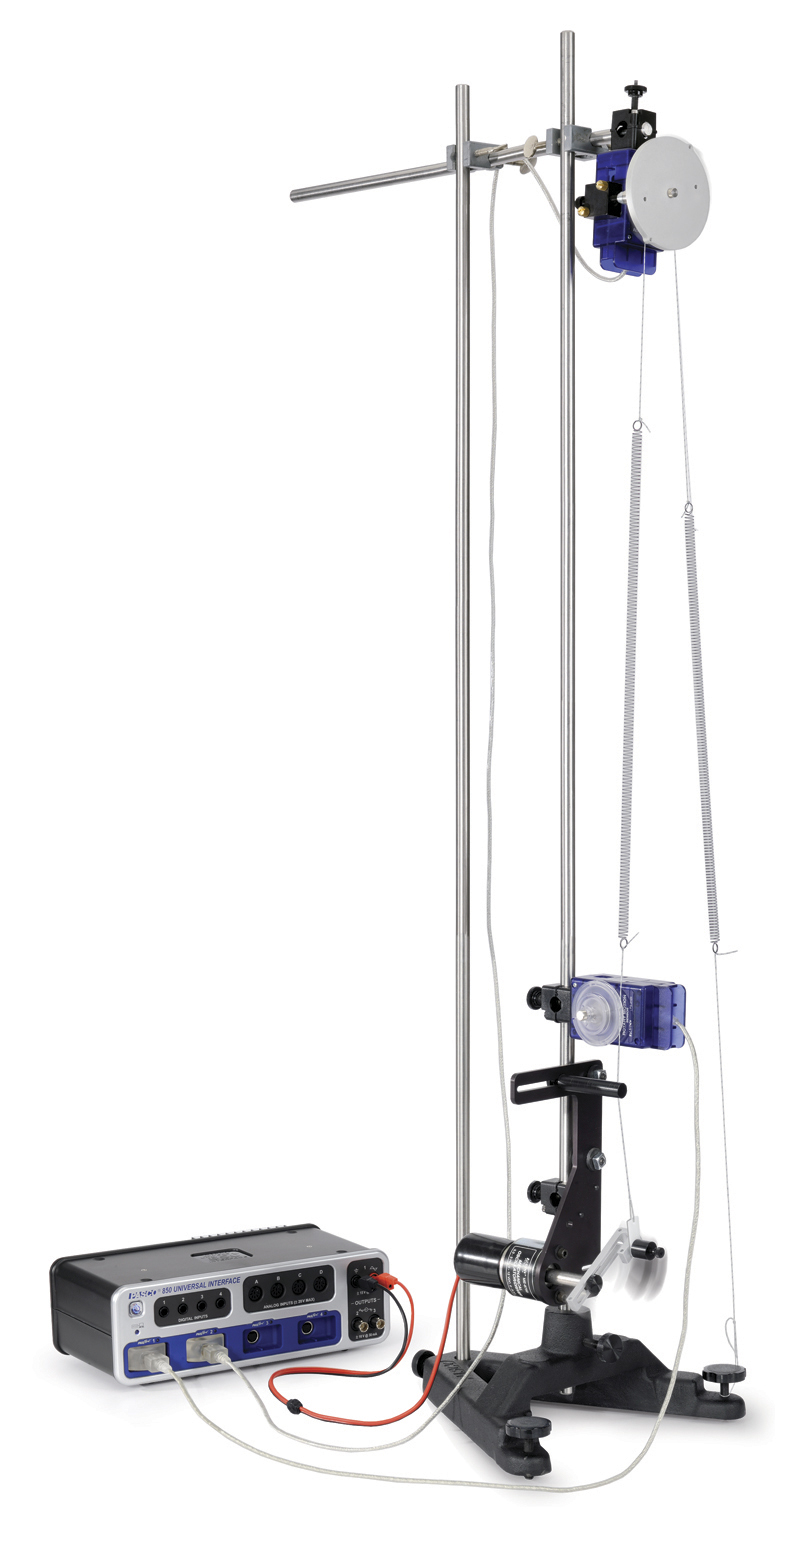
\includegraphics[width=\linewidth]{set}
		\caption{Equipment Setup}
	\end{minipage}
	\hfill
	\begin{minipage}[c]{0.5\linewidth}
		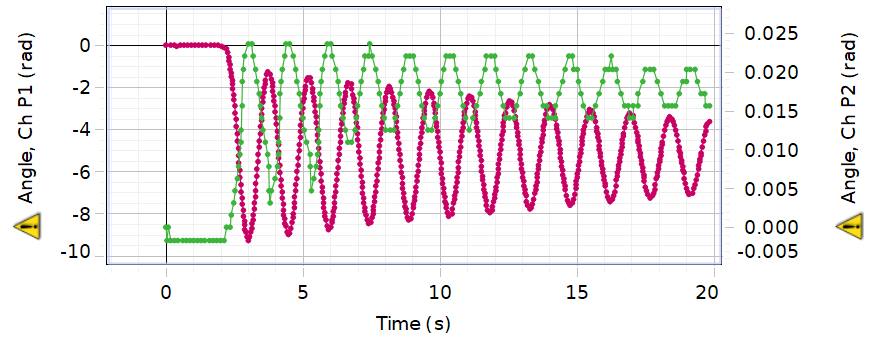
\includegraphics[width=\linewidth]{sign}
		\caption{Two Sensors Should Read Same Sign}
	\end{minipage}%
\end{figure}


\section{Procedure}
\subsection{Parameters Collection}
The radius $(r)$ and mass $(M)$ of the disk was measured before the experiment began.
\begin{equation}
\begin{aligned}
r &= 4.7600 \pm 0.0025 \text{ cm}\\
M &= 121.32 \pm 0.01 \text{ g}
\end{aligned}
\end{equation}
The mass of a golden cylinder ($m$) was also measured.
\begin{equation}
m = 14.59\pm0.01\text{ g}
\end{equation}

\subsection{Undamped Frequency}
We cranked the magnet all the way back to minimize the magnetic damping. The disk was displaced and set free to oscillate. Curve fitting of the angular displacement plot gave the undamped angular frequency
\begin{equation}
\omega_{\text{exp}} = 4.28 \pm 2.5\times10^{-4}\text{ Hz}
\end{equation}
Since the error from the fitting was rather small, we chose to neglect it and directly obtained the undamped frequency by
\begin{equation}
f_{\text{exp}} = \frac{\omega}{2\pi}= 0.68\text{ Hz}
\end{equation}
\begin{figure}[h]\centering{
		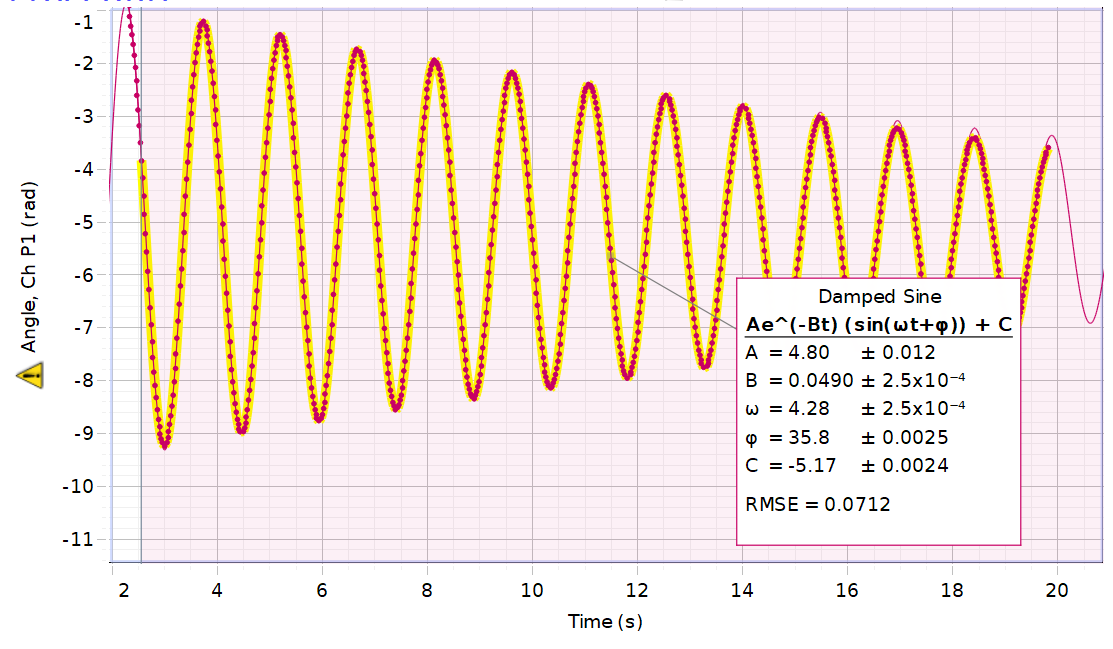
\includegraphics[width=0.8\linewidth]{r}}
	\caption{$\theta-t$ with Minimal Damping}
\end{figure}

\subsection{Torsion Coefficient}
The golden cylinder with known mass $m$ and radius $r$ was hung on top of one spring. The resulting angular displacement of the disk was recorded to be (see Figure 4)
\begin{equation}
\theta = 1.083 \pm 0.001 \text{ rad}
\end{equation}
Using equation (1) we obtained the torsion coefficient
\begin{equation}
\begin{aligned}
\kappa &= \frac{\tau}{\theta}= \frac{mgr}{\theta}\\
&= 0.6284 \pm 0.0008 \text{ N cm}
\end{aligned}
\end{equation}
where the uncertainty was given by
\begin{equation}
\delta_{\kappa} = g\sqrt{(r\delta_m/\theta)^2+(m\delta_r/\theta)^2+(mr\delta_\theta/\theta^2)^2
}
\end{equation}

\begin{figure}[h]\centering{
		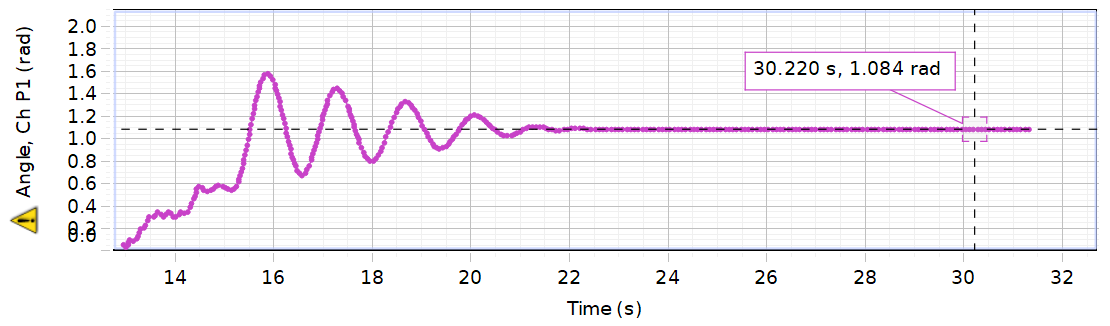
\includegraphics[width=\linewidth]{sprconst}}
	\caption{Measuring Torsion Coefficient}
\end{figure}

\subsection{Rotational Inertia}
The moment of inertia of the disk was calculated by
\begin{equation}
I = \frac12Mr^2=1374.41\pm1.45\text{ g cm}^2
\end{equation}
where the uncertainty was given approximated by the propagation error
\begin{equation}
\delta_I = \sqrt{
	\delta_M^2r^4/4+M^2r^2\delta_r^2
}
\end{equation}

\subsection{Resonance Curves}
We placed the magnet 5 mm from the disk and slowly varied the driving frequency from around 1 Hz to 0.5 Hz. The resulting amplitude of oscillation was plotted against the driving frequency. Similar plots were generated after adjusting the magnet to 4 mm and 3 mm off the disk (See Figure 5).

\subsection{Damping Coefficient}
For the 3 mm damping, we recorded the amplitude of the disk as the system damped out in time. A damped sine fitting was conducted to determine the damping coefficient $b$.
\begin{figure}[h]\centering{
		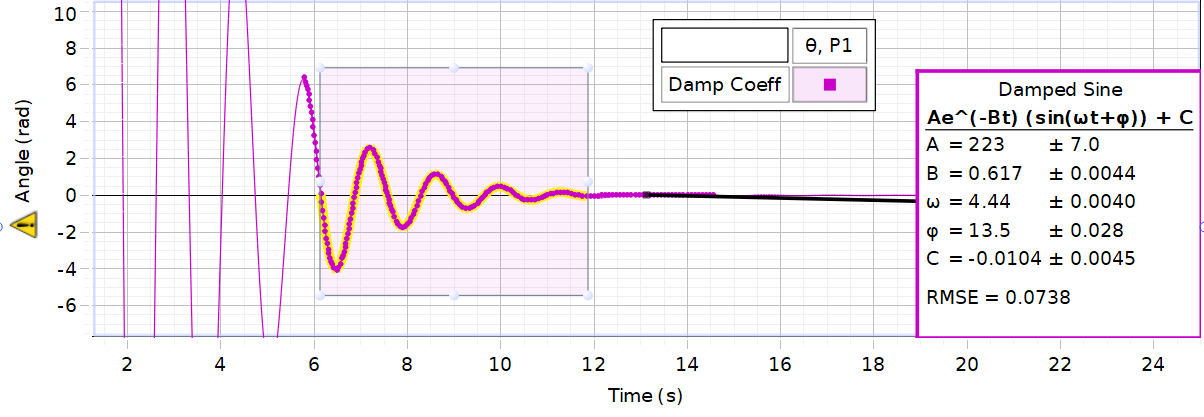
\includegraphics[width=\linewidth]{coeff}}
	\caption{Finding Damping Coefficient}
\end{figure}
Comparing the fitted curve with equation (3), we obtained
\begin{equation}
\begin{aligned}
\frac{b}{2I} &= 0.617 \pm 0.004 \text{ m}^{-2} \text{s}^{-1}\\
b &= 0.1696 \pm 0.0012 \text{ g/s}
\end{aligned}
\end{equation}

\section{Analysis}
\subsection{Theoretical vs. Experimental Undamped Frequencies}
We used the values of $\kappa$ and $I$ obtained respectively in (19) and (21) to calculate the theoretical undamped frequency
\begin{equation}
\begin{aligned}
f_0 &= \frac{2\pi}{\sqrt{\kappa/I}}\\
&= 0.93\pm7.68\times10^{-4} \text{ Hz}
\end{aligned}
\end{equation}
where the uncertainty was given by
\begin{equation}
\delta_{f_0} = \pi\sqrt{\delta^2_I/\kappa I+\delta^2_\kappa I/\kappa^3}
\end{equation}
Note that the experimental value obtained previously was significantly lower compared to the theoretical value, with a percentage difference of
\begin{equation}
\frac{f_{\text{exp}} - f_0}{f_0}= -26.88\%
\end{equation}
This was because, despite having minimized the magnetic damping, external damping caused by frictional drag was still present throughout the experiment. This means that the damping term $b^2/4I^2$ in
\begin{equation}
\omega = \sqrt{\omega_0^2-b^2/4I^2}
\end{equation}
was in fact greater than zero due to friction, resulting in a lower experimental frequency. 

\subsection{Analysis of Resonance Curves}
Examining the resonance curves, we found that increasing damping (smaller distance) results in a decreasing amplitude at resonance. This was consistent with the theory that the resonant amplitude decreases monotonically with $b$ in significant underdamping.


However, the resonant frequency remained mostly unchanged with different amounts of damping, which seemed to be inconsistent with equations (9). In theory, the resonant (angular) frequency 
\begin{equation}
\omega_r = \sqrt{\omega_0^2-2(b/I)^2}
\end{equation}
should decrease monotonically as the damping increases. An explanation of this discrepancy could be that the change in the damping coefficient $b$ by adjusting the position of the magnet was too small to produce noticeable difference in $\omega_r$. Another explanation could be that the setup of the equipment or the accuracy of the measurement was not ideal enough to replicate the theory.
\begin{figure}[h]
	\begin{minipage}[c]{0.46\linewidth}
		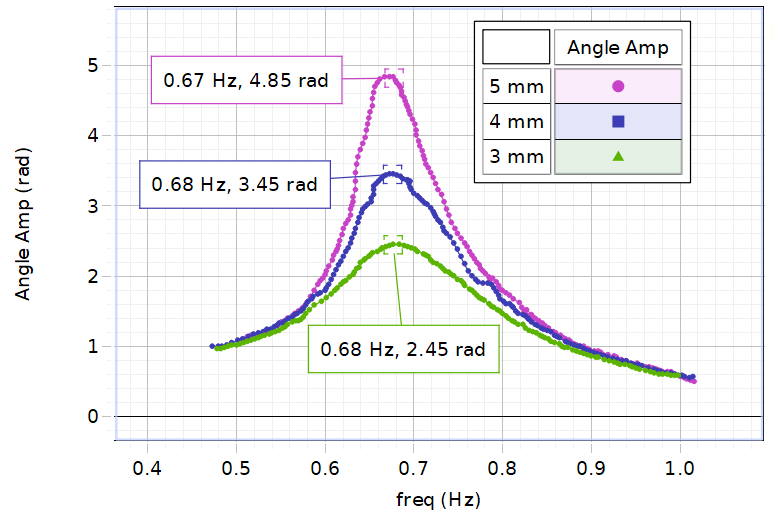
\includegraphics[width=\linewidth]{res}
		\caption{Experimental Curves of Amplitude (rad) vs. Driving Frequency (Hz) for Different Amounts of Magnetic Damping}
	\end{minipage}
	\hfill
	\begin{minipage}[c]{0.48\linewidth}
		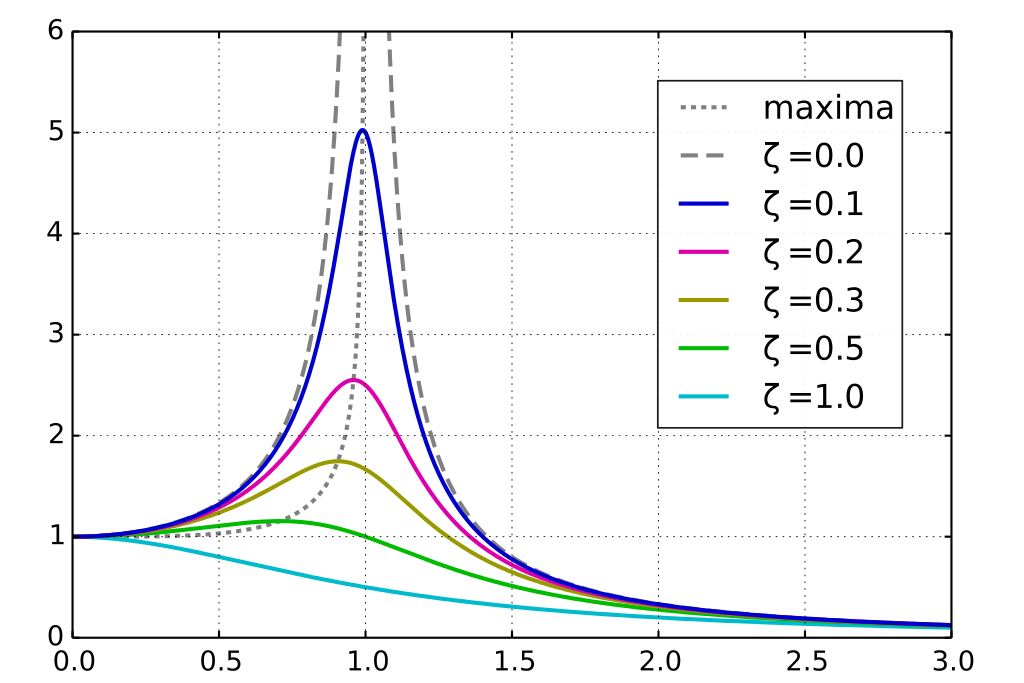
\includegraphics[width=\linewidth]{theo}
		\caption{Theoretical Curves of Amplitude (rad) vs. Relative Driving Frequency $\omega/\omega_0$ 
			\\($\zeta \propto b$ is the damping ratio)}
	\end{minipage}%
\end{figure}

It was also noted that all resonance curves were asymmetric about the resonant frequencies. This was due to the asymmetry in the behaviors of the response amplitude as the driving frequency approaches 0 and $\infty$ Hz. Specifically, as the driving frequency approaches zero, the resulting amplitude approaches 1 rad. However as the driving frequency approaches infinity, the response amplitude approaches 0 rad.
\subsection{Fitting Theory to Resonance Curve}
We fit the resonance curve of 3 mm damping with a function of the form of equation (9). Since the resonance curve has the regular frequency as its $x$ coordinate, we rewrote equation (9) as
\begin{equation}
\theta_0(f) = \frac{\tau_0/I}{2\pi\sqrt{4\pi^2(f^2-f_0^2)+(fb/I)^2}}
\end{equation}
The fitting yielded
\begin{equation}
\begin{aligned}
f_0 &= 0.704 \text{ Hz}\\
b &= 1.39 \text{ g/s}
\end{aligned}
\end{equation}

\begin{figure}[h]\centering{
		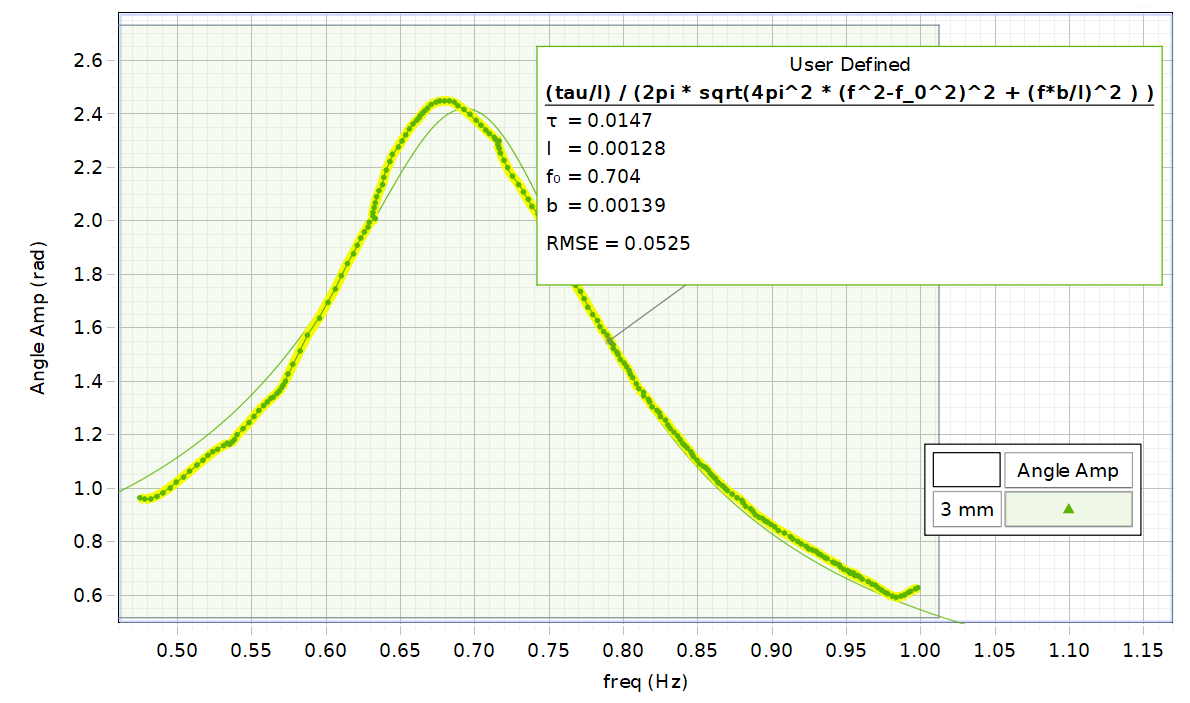
\includegraphics[width=0.75\linewidth]{fit}}
	\caption{Fitting Resonance Curve of 3 mm Damping}
\end{figure}

\subsection{Phase Analysis}
The phase difference of the driver velocity and the disk velocity was approximately $\pi$ at the beginning (when $\omega$ was highest), $\pi/2$ around the resonance, and was approaching $0$ in the end (when $\omega$ was lowest). This agreed well with the theory.

\begin{figure}[h]\centering{
		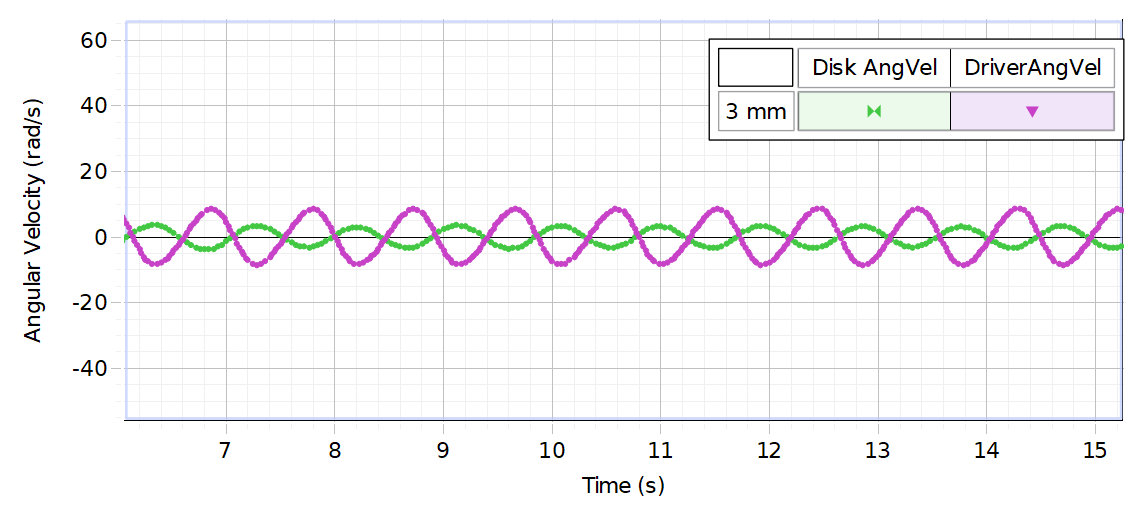
\includegraphics[width=0.75\linewidth]{1}}
	\caption{$\phi\approx\pi$ at High Driving Frequencies}
\end{figure}
\begin{figure}[h]\centering{
		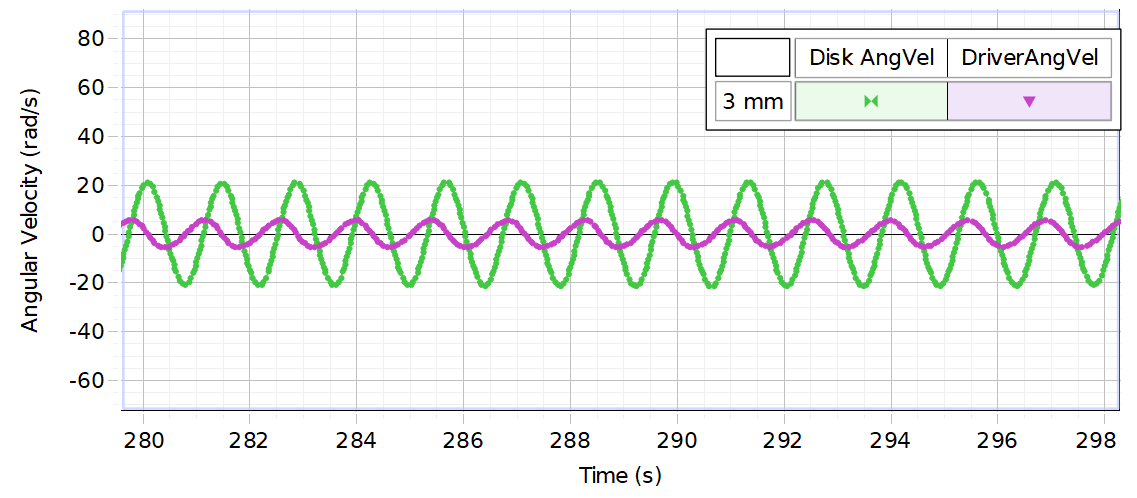
\includegraphics[width=0.75\linewidth]{2}}
	\caption{$\phi\approx\pi/2$ around Resonance}
\end{figure}
\begin{figure}[h]\centering{
		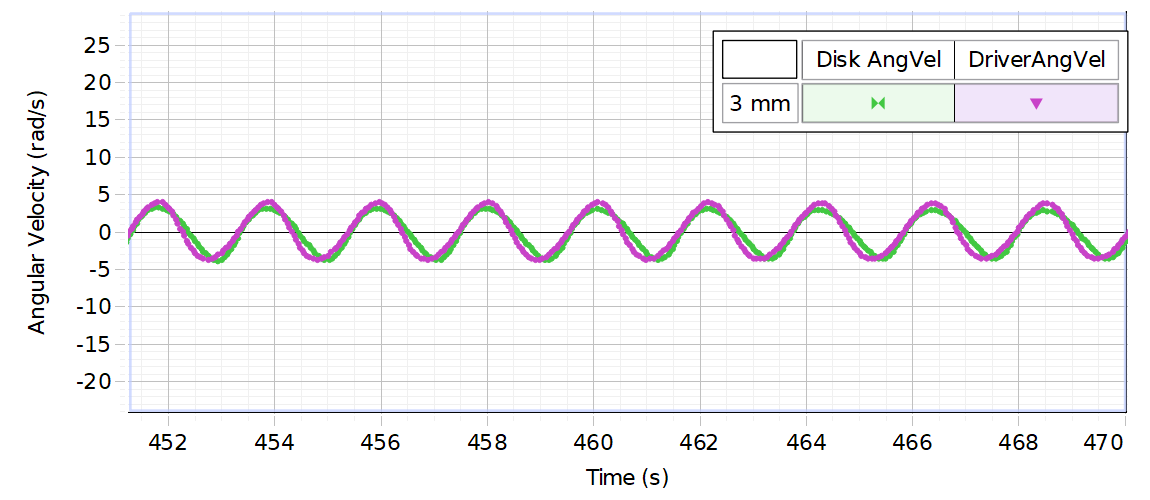
\includegraphics[width=0.75\linewidth]{3}}
	\caption{$\phi\approx0$ at Low Driving Frequencies}
\end{figure}

\end{document}